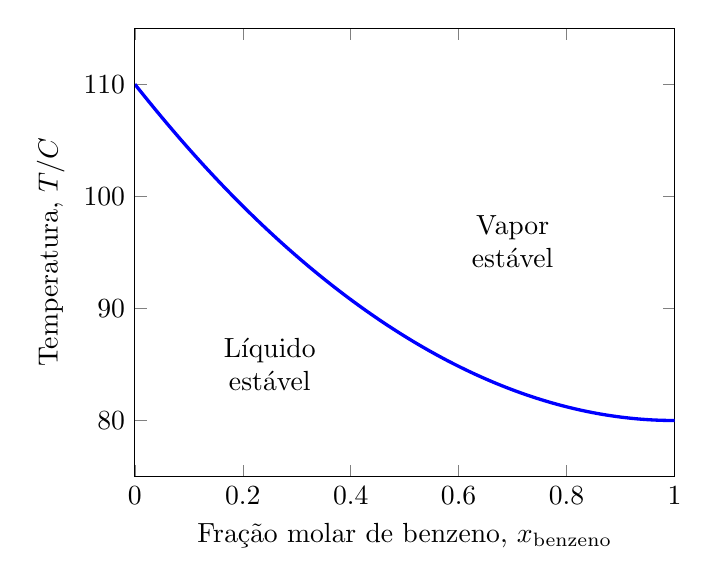
\begin{tikzpicture}
\begin{axis}
    [
        grid = minor,
        xlabel = {Fração molar de benzeno, $x_\mathrm{benzeno}$},
        ylabel = {Temperatura, $T/\unit{\degree C}$},
        xmin = 0, xmax = 1,
        ymin = 75, ymax = 115,
    ]    
    \draw [draw=blue, very thick]
        (axis cs: 0, 110) parabola bend  (axis cs: 1, 80)
        (axis cs: 1, 80); 

    \node [align = center] at (axis cs:0.25, 85) 
            { Líquido\\estável };

    \node [align = center] at (axis cs:0.7, 96) 
            { Vapor\\estável };
\end{axis}
\end{tikzpicture}